\chapter{Parameter Estimation}
\label{chap:parameter-estimation}
\thispagestyle{empty}

Let us now compare the $\Lambda$CDM- and DGP-model. To do this, we will consider the ``Union2.1'' SN Ia compilation and determine best-fit values for the parameter pair ($\Omega_{\text{m},0}$, $\Omega_{\Lambda,0}$) in $\Lambda$CDM- and ($\Omega_{\text{m},0}$, $\alpha$) in DGP-model by computing the $\chi^2$-distribution, which is a measure for the likelihood.

\section{Supernovae Type Ia ``Union2.1'' Dataset}

\noindent The SN Ia ``Union2.1'' dataset (see appendix \ref{app:dataset-and-source-codes}) used in this thesis contains the name, the redshift, the distance modulus, and the distance modulus error of 580 supernovae, measured by the Hubble Space Telescope. \\

\noindent First, let us have a look at the dataset. We plot the distance modulus (see Equation \eqref{eq:distance-modulus}) $m - M$ against the redshift $z$ for the predicted luminosity distance $d_{\text{L}}$ by the $\Lambda$CDM-model with $(\Omega_{\text{m},0}, \Omega_{\Lambda,0}) = (0.3, 0.7)$ and DGP-model with $(\Omega_{\text{m}}, \alpha)=(0.3, 1.0)$.

\begin{figure}[H]
   \centering
   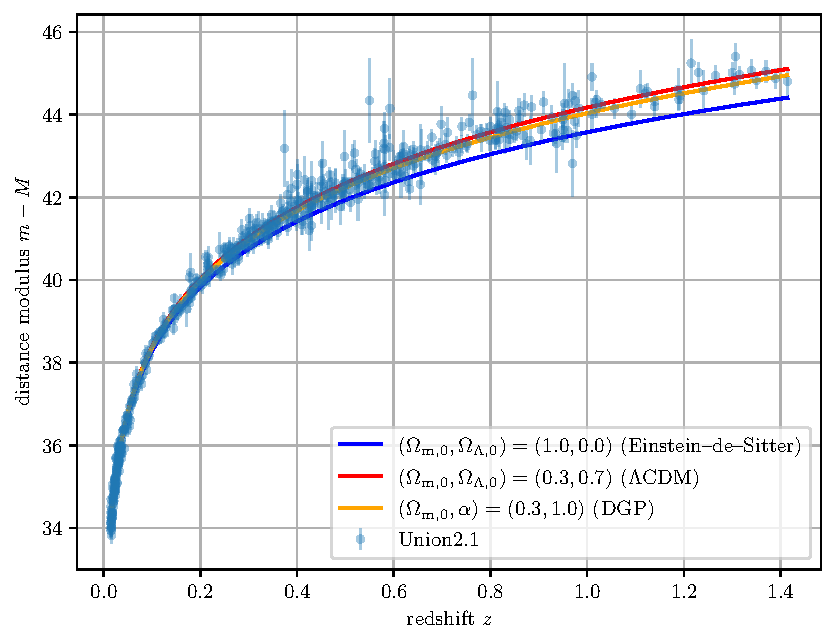
\includegraphics[scale=0.97]{figures/plots/PDF/redshift-vs-distance-modulus.pdf}
   \caption{Distance modulus $m - M$ against redshift $z$ for Einstein--de--Sitter-model $(\Omega_{\text{m},0}, \Omega_{\Lambda,0}) = (1.0, 0.0)$, the $\Lambda$CDM-model with $(\Omega_{\text{m},0}, \Omega_{\Lambda,0}) = (0.3, 0.7)$ and DGP-model with $(\Omega_{\text{m},0}, \alpha) = (0.3, 1.0)$.\\}
   \label{fig:redshift-vs-distance-modulus}
\end{figure}

\noindent At first sight, we see that a universe that contains only matter (Einstein--de--Sitter-model) cannot match the data, especially for high redshifts. \\
Further, we can conclude that the data points at high redshift ($z \gtrsim 0.8$) have a greater influence on the fit for the estimated parameters, since there is no significant fluctuation of data points at low redshift. \\
The apparently large errors of some data points in the range of $0.35 \leq z \leq 1.0$ should not cause any concerns whether this dataset is suitable for an adequate parameter estimation, since the error of low-redshift data points will impact the fit to a lesser degree than errors in high-redshift data points.

\section{Statistical Analysis}
To obtain values for the best-fit parameters, we consider the distance of every data point between its \textit{measured} relative magnitude to the \textit{theoretical} value the relative magnitude would have dependent on the parameters of the model. \\ 
From now on, we denote $\vb*{\theta}$ as the parameter pairs of the model we want to estimate, so 
\begin{align}
    \vb*{\theta} = \begin{cases}
                        (\Omega_{\text{m},0}, \Omega_{\Lambda,0}) &\text{for $\Lambda$CDM-model}\\
                        (\Omega_{\text{m},0}, \alpha)             &\text{for DGP-model}\\
                   \end{cases}. \label{eq:cosmological-parameters}
\end{align}
The given dataset is a sample of $N = 580$ datapoints which contain for datapoint $i \in [1,N]$ the redshift $z_{i}$, the distance modulus and therefore implicitly\footnote{Although the ``Union2.1'' SN Ia compilation contains the distance modulus $m - M$, we will handle it throughout the parameter estimation as if it only contains the relative magnitude $m$. Since we are going to marginalize the parameter $M$, it has no influence on the parameter estimation.} the relative magnitude $m_{i}$ and its error $\sigma_{m_{i}}$. \\
Our goal is to express the quantities given \textit{only} through the free parameters $\vb*{\theta}$. \\
Now, let us consider the relative magnitude $m$, which is given by the distance modulus (see Equation \eqref{eq:distance-modulus}). First, we want to express the luminosity distance $d_{\text{L}}$ in multiples of $\SI{1}{\mega \parsec}$, so we obtain
\begin{align*}
    m &= M + 5\log_{10}\biggl( \frac{d_{\text{L}}}{\SI{10}{\parsec}} \biggr) = M + 5\log_{10}\biggl( 10^{5} \frac{d_{\text{L}}}{\SI{1}{\mega \parsec}} \biggr) \\
      &= M + 25 + 5\log_{10}\biggl(\frac{d_{\text{L}}}{\SI{1}{\mega \parsec}}\biggr). 
\end{align*}
Since the luminosity distance $d_{\text{L}}$ depends on the Hubble distance $d_{\text{H}}$ (see Equation \eqref{eq:comoving-distance} and \eqref{eq:luminosity-distance}) and is therefore proportional to $d_{\text{L}} \propto 1/H_{0}$, we redefine the luminosity distance so that it is independent of the Hubble constant. Hence, we go on with 
\begin{align}
m &= M + 25 + 5\log_{10} \biggl(\frac{1}{H_{0}} H_{0} d_{\text{L}}(z, H_{0}, \vb*{\theta}) \SI{}{\mega \parsec^{-1}} \biggr) \nonumber \\
  &= \underbrace{M + 25 - 5\log_{10}(H_{0})}_{ =: \mathcal{M}(H_{0}) } + 5 \log_{10} \biggl( \underbrace{H_{0} d_{\text{L}}(z, H_{0}, \vb*{\theta})}_{ =: \mathcal{D}_{\text{L}}(z, \vb*{\theta}) } \SI{}{\mega \parsec^{-1}} \biggr) \nonumber \\
  &= \mathcal{M}(H_{0}) + 5 \log_{10}(\mathcal{D}_{\text{L}}(z, \vb*{\theta}) \SI{}{\mega \parsec^{-1}}). \label{eq:relative-magnitude_mod-magnitude_mod-luminosity-distance}
\end{align}
With Equation \eqref{eq:relative-magnitude_mod-magnitude_mod-luminosity-distance}, the dependency on the Hubble constant is now in an additive constant $\mathcal{M}(H_{0})$, which will be useful as we see later. \\

\noindent From now on, we are going to call the relative magnitude in Equation \eqref{eq:relative-magnitude_mod-magnitude_mod-luminosity-distance} the \textit{theoretical} relative magnitude $m_{\text{th}}$, since it contains the cosmological parameters $\vb*{\theta}$. \\ 

\noindent Given the dataset $D := \{z_{i}, m_{i}, \sigma_{m_{i}} \}$, where $z_{i}$ is the measured redshift, $m_{i}$ the measured relative magnitude and $\sigma_{m_{i}}$ the error of the relative magnitude $m_{i}$, we define 

\begin{align}
    \chi^2(\mathcal{M}, \vb*{\theta} \vert D) := \sum_{i=1}^{N} \biggl(\frac{m_{\text{th}}(z_{i}, \mathcal{M}, \vb*{\theta}) - m_{i}}{\sigma_{m_{i}}}\biggr)^2 \label{eq:chi-square} 
\end{align}
as the $\chi^2$-distribution of $\mathcal{M}$ and $\vb*{\theta}$. \\
\noindent The likelihood, which is a probability density, is given by 
\begin{align}
    L(\mathcal{M}, \vb*{\theta} \vert D) := L_{0} \exp \biggl(-\frac{1}{2} \chi^2(\mathcal{M}, \vb*{\theta} \vert D) \biggr),  \label{eq:likelihood}
\end{align}
where $L_{0}$ is a normalization factor.
With the likelihood $L$, it is possible to calculate the probability $P$ to find $\mathcal{M} \in \mathcal{I}_{\mathcal{M}}$ and $\vb*{\theta} \in \mathcal{I}_{\vb*{\theta}}$ in a parameter interval $\mathcal{I}_{\mathcal{M}}$ and $\mathcal{I}_{\vb*{\theta}}$ with 

\begin{align}
    P(\mathcal{M} \in \mathcal{I}_{\mathcal{M}}, \vb*{\theta} \in \mathcal{I}_{\vb*{\theta}} \vert D) = \int\limits_{\mathcal{I}_{\mathcal{M}}} \dd{\mathcal{M}} \int\limits_{\mathcal{I}_{\vb*\theta}} \dd{\vb*{\theta}} L(\mathcal{M}, \vb*{\theta} \vert D). \label{eq:probability}   
\end{align}
However, this probability $P$ still depends on $\mathcal{M}$, which is not measured. Since our goal is to find the best-fit values for $\vb*{\theta}$ and therefore express the probability only through $\vb*{\theta}$, we are going to \textit{marginalize} over $\mathcal{M}$. We obtain the \textit{marginalized} likelihood $L_{\text{M}}$ by integrating the likelihood $L$ over all possible values that $\mathcal{M}$ could take. Assuming $\mathcal{M} \in (-\infty, \infty)$, it follows  
\begin{align}
    L_{\text{M}}(\vb*{\theta} \vert D) = \int\limits_{-\infty}^{\infty} \dd{\mathcal{M}} L(\mathcal{M}, \vb*{\theta} \vert D). \label{eq:marginalized-likelihood} 
\end{align}
Thereby, we can calculate the probability $P(\vb*{\theta} \in \mathcal{I}_{\vb*{\theta}} \vert D)$ to find values for $\vb*{\theta} \in \mathcal{I}_{\vb*{\theta}}$, given the dataset $D$, but without any information on $\mathcal{M}$, which implicitly contains the Hubble constant $H_{0}$, so
\begin{align}
    P(\vb*{\theta} \in \mathcal{I}_{\vb*{\theta}} \vert D) = \int\limits_{\mathcal{I}_{\vb*{\theta}}} \dd{\vb*{\theta}} L_{\text{M}}(\vb*{\theta} \vert D). \label{eq:marginalized-probability}
\end{align}
Since $\mathcal{M}$ is only an additive constant (see Equation \eqref{eq:relative-magnitude_mod-magnitude_mod-luminosity-distance}), this can be done analytically. To do so, we set $\mathcal{M} = 0$ and introduce the terms
\begin{align}
    c_{1}(\{\sigma_{m_{i}} \}) &:= \sum_{i = 1}^{N} \frac{1}{\sigma_{m_{i}}^2}, \\
    b_{0}(\vb*{\theta} \vert D) &:= \sum_{i = 1}^{N} \frac{m_{\text{th}}(z_{i}, \vb*{\theta}) - m_{i}}{\sigma_{m_{i}}^2}, \\
    b_{1}(\vb*{\theta} \vert D) &:= \sum_{i = 1}^{N} \biggr(\frac{m_{\text{th}}(z_{i}, \vb*{\theta}) - m_{i}}{\sigma_{m_{i}}} \biggl)^2,
\end{align}
by which we obtain
\begin{align}
    \chi^2 (0, \vb*{\theta} \vert D) = b_{1}(\vb*{\theta} \vert D) - \frac{b_{0}^2 (\vb*{\theta} \vert D)}{c_{1}(\{ \sigma_{m_{i}} \})} =: \chi_{\text{A}}^2 (\vb*{\theta} \vert D) \label{eq:analytic-chi-square} 
\end{align}
and thus for the likelihood
\begin{align}
    L(0, \vb*{\theta} \vert D) = L_{0} \exp \biggl(-\frac{1}{2} \chi_{\text{A}}^2(\vb*{\theta} \vert D) \biggr) =: L_{\text{A}}(\vb*{\theta} \vert D). \label{eq:analytic-likelihood} 
\end{align}
The expressions $L_{\text{M}}$ (see Equation \eqref{eq:marginalized-likelihood}) and $L_{\text{A}}$ (see Equation \eqref{eq:analytic-likelihood}) lead to the same results, which we will check later for a minimal working example in the case of the $\Lambda$CDM-model. In the following, we denote the likelihood and the $\chi^2$-distribution that are independent of $\mathcal{M}$ simply as $L(\vb*{\theta} \vert D)$ and $\chi^2(\vb*{\theta} \vert D)$. 

\noindent The best-fit parameters $\vb*{\theta}_{\text{best}}$ are located at the maximum of the likelihood, so 
\begin{align}
    \pdv{L(\vb*{\theta} \vert D)}{\vb*{\theta}} \bigg \vert_{\vb*{\theta}_{\text{best}}} = 0.
\end{align}

\noindent Since $L(\vb*{\theta} \vert D)$ is a concave function of $\chi^2(\vb*{\theta} \vert D)$, we can find the best-fit parameters $\vb*{\theta}_{\text{best}}$ at the minimum of $\chi^2(\vb*{\theta} \vert D)$. The $\chi^2$-distribution is a measure for the so called \textit{log-likelihood}, which is sometimes considered rather than the likelihood for practical purposes and convenience of computational work. However, this has no influence on the outcome of the parameter estimation. \\

\noindent After we obtain $\vb*{\theta}_{\text{best}}$, it is important to find the $\sigma_{\vb*{\theta}}$-regions, which make a statement about the probability to find $\vb*{\theta}$ in a certain parameter interval\footnote{The interval $\mathcal{I}_{n \sigma_{\vb*{\theta}}}$ is sometimes called the ``confidence interval''.}  $\mathcal{I}_{n\sigma_{\vb*{\theta}}} \subset \mathcal{I}_{\vb*{\theta}}$. Their construction is based on the standard deviation $\sigma_{x}$ of a Gaussian distribution
\begin{align}
    g(x \vert \mu_{x}, \sigma_{x}) = \frac{1}{\sqrt{2\pi} \sigma_{x}} \exp \biggl[- \frac{1}{2} \biggl(\frac{x - \mu_{x}}{\sigma_{x}} \biggr)^2 \biggr], \label{eq:gauss-distribution} 
\end{align}
where $\mu_{x}$ is the mean of $x$ and $\sigma_{x}^2$ the variance of $x$, so that the probability of finding \\ 
${x \in[\mu_{x} - n\sigma_{x}, \mu_{x} + n \sigma_{x}] =: \mathcal{I}_{n\sigma_{x}}, n \in \N}$ is given by
\begin{align}
    P(x \in \mathcal{I}_{n\sigma_{x}} \vert \mu_{x}, \sigma_{x}) = \int\limits_{\mathcal{I}_{n\sigma_{x}}} \dd{x} g(x \vert \mu_{x}, \sigma_{x}) =: P_{n\sigma_{x}}
\end{align}
and therefore
\begin{align}
    P(\vb*{\theta} \in \mathcal{I}_{n \sigma_{\vb*{\theta}}} \vert D) = \int\limits_{\mathcal{I}_{n \sigma_{\vb*{\theta}}}} \dd{\vb*{\theta}} L(\vb*{\theta} \vert D) = P_{n \sigma_{x}}.  
\end{align}

\noindent It is common to express statistical accuracies in multiples of the standard deviation. 
To calculate $P_{n\sigma_{x}}$, let us take a step back to the meaning of the $\chi^2$-distribution. In general, the $\chi_{k}^{2}$-distribution is defined to be proportional to the sum of the squares of $k$ statistically independent, standard normal distributed random variables $X_{i}$ ($i \in [1,k]$), so
\begin{align}
    P(X_{1}, ..., X_{k}) = \prod_{i = 1}^{k} P(X_{i}) \land X_{i} \sim g(x \vert 0, 1) \Rightarrow  \sum_{i = 1}^{k} X_{i}^2 \sim \chi_{k}^2. 
\end{align}
The $\chi_{k}^{2}$-distribution depends on the amount of statistically independent random variables $k$, which is often called the \textit{degree of freedom}. \\
The probability density function (``PDF'') of the $\chi_{k}^{2}$-distribution is given by
\begin{align}
    f_{k}(x) = \frac{1}{2^{\frac{k}{2}} \Gamma (\tfrac{k}{2})} x^{\frac{k}{2} - 1} \E^{-\frac{1}{2}x} \quad \text{for} \quad x > 0, \label{eq:probability-density-function}
\end{align}
where 
\begin{align}
    \Gamma(s) := \int\limits_{0}^{\infty} \dd{t} t^{s - 1} \E^{-t} \label{eq:gamma-function}  
\end{align}
is the gamma function. \\
The cumulative density function (``CDF'') of the $\chi_{k}^{2}$-distribution is given by 
\begin{align}
    F_{k}(x) = \frac{1}{\Gamma(\tfrac{k}{2})} \gamma(\tfrac{k}{2}, \tfrac{x}{2}) = \frac{1}{\Gamma(\tfrac{k}{2})} \int\limits_{0}^{\frac{x}{2}} \dd{t} t^{\frac{k}{2} - 1} \E^{-t} \quad \text{for} \quad x > 0, \label{eq:cumulative-distribution-function}
\end{align}
where $\gamma(\tfrac{k}{2}, \tfrac{x}{2})$ is the lower incomplete gamma function. \\
The values of $P_{n \sigma_{x}}$ can be computed by 
\begin{align}
    P_{n \sigma_{x}} = F_{1}(n^2) = \frac{1}{\Gamma(\tfrac{1}{2})} \int\limits_{0}^{\frac{n^2}{2}} \dd{t} t^{-\frac{1}{2}} \E^{-t}. 
\end{align}
Since $\vb*{\theta}$ contains for both cosmological models two parameters (see Equation \eqref{eq:cosmological-parameters}), the $\chi^2$-distribution that only depends on $\vb*{\theta}$ has $k = 2$ degrees of freedom, which leads to the probability density function 
\begin{align}
    f_{2}(x) = \frac{1}{2} \E^{-\frac{1}{2}x} \quad \text{for} \quad x > 0 \label{eq:probability-density-function-2} 
\end{align}
and the cumulative density function 
\begin{align}
    F_{2}(x) = 1 - \E^{-\frac{1}{2}x} \quad \text{for} \quad x > 0. \label{eq:cumulative-density-function-2} 
\end{align}
The quantile function, sometimes called ``percent-point function'' (``PPF'') or ``inverse cumulative distribution'', $Q(P)$ returns the value $x$ of a random variable $X$ for the probability $P$ to find $X \leq x$. With the cumulative distribution function $F_{2}(x)$, the quantile function $Q(P)$ is 
\begin{align}
    Q(P) = -2 \ln(1 - P). \label{eq:quantile-function} 
\end{align}
For $P_{n \sigma_{x}}$, we define 
\begin{align}
    Q_{n} := -2 \ln(1 - P_{n \sigma_{x}}). \label{eq:quantile-function-n} 
\end{align}
The $\sigma_{\vb*{\theta}}$-regions satisfy the condition
\begin{align}
    \forall \vb*{\theta} \in \mathcal{I}_{n \sigma_{\vb*{\theta}}}: L(\vb*{\theta} \vert D) = L_{0} \exp \biggl[-\frac{1}{2} \biggl(\chi^{2}(\vb*{\theta}_{\text{best}} \vert D) + Q_{n} \biggr)\biggr]. \label{eq:sigma-regions-condition} 
\end{align}


\section{Computational Implementation and Results}

The source codes which are subject to this analysis are written in Python. \\
The main computational implementations that lead to the following results are only outlined for a minimal working example in the case of the $\Lambda$CDM-model. For a full insight to the entire source codes that are used to produce the plots and the results in this thesis, see appendix \ref{app:dataset-and-source-codes}. \\

\subsection{$\Lambda$CDM-Model}

\subsubsection{Minimal Working Example -- $\Lambda$CDM-Model for a Flat Universe ($\Omega_{k,0} = 0$)}
Before writing huge and complex code, it is always a good idea to reduce the complexity of the cosmological model by creating a simple, minimalistic ``toy model''.
To do so for the $\Lambda$CDM-model, we assume a flat universe (and, as mentioned on page~\pageref{no-radiation}, no radiation) -- so $\Omega_{k,0} = 0$ (and $\Omega_{\text{r},0} = 0$). \\
With Equation \eqref{eq:density-parameters-sum} follows $\Omega_{\Lambda,0} = 1 - \Omega_{\text{m},0}$ and therefore with Equation \eqref{eq:scale-factor-redshift-relation} for the expansion function (see Equation \eqref{eq:expansion-function})
\begin{align}
    E(z) = \sqrt{\Omega_{\text{m},0}(1 + z)^3 + 1 - \Omega_{\text{m},0}}. \label{eq:expansion-function-flat-universe} 
\end{align}
In the case of a flat universe, the comoving distance is simply given by $d_{\text{C}} = d_{\text{H}} I$, where $I$ is the expression \eqref{eq:expansion-integral} with the expansion function in Equation \eqref{eq:expansion-function-flat-universe}. With Equation \eqref{eq:luminosity-distance} and \eqref{eq:relative-magnitude_mod-magnitude_mod-luminosity-distance}, the (modified) luminosity distance $\mathcal{D}_{\text{L}}$ for our simplified model is 
\begin{align}
    \mathcal{D}_{\text{L}}(z, \Omega_{\text{m},0}) = (1 + z) c \int\limits_{0}^{z} \dd{z'} \frac{1}{\sqrt{\Omega_{\text{m},0}(1 + z')^3 + 1 - \Omega_{\text{m},0}}}. \label{eq:modified-luminosity-distance-flat-universe} 
\end{align}
A computational implementation of those functions could look as in Listing \ref{lst:MWE-expansion-function-and-modified-luminosity-distance}.

\begin{lstlisting}[language=Python, caption={Function for $E(z)$ and $\mathcal{D}_{\text{L}}(z, \Omega_{\text{m},0})$.}, label={lst:MWE-expansion-function-and-modified-luminosity-distance}]
def expansion_function(z, Omega_m0):
    return np.sqrt(Omega_m0 * np.power(1.0 + z, 3) + 1.0 - Omega_m0)


def integrand(z, Omega_m0):
    if z == 0.0:
        return 1.0
    E = expansion_function(z, Omega_m0)
    return 1.0/E


def integral(z, Omega_m0):
    # d_C/d_H = Integrate[1/E(z'), {z',0,z}]
    return quad(integrand, 0.0, z, args=(Omega_m0,))[0]


def mod_luminosity_distance(z, Omega_m0):
    # Cosmological Parameters
    # =======================
    c = 299792.458           # speed of light in vacuum in km/s
    H_0 = 1.0                # dependence on hubble constant is set into mod_absolute_magnitude
    d_H = c/H_0              # hubble distance
    # =======================
    
    I = np.array([integral(zi, Omega_m0)  for zi in z])
   
    return (1.0 + z) * d_H * I
\end{lstlisting}
The function \colorbox{backcolor}{\lstinline{quad}}, which is returned by \colorbox{backcolor}{\lstinline{integral}}, is imported from \colorbox{backcolor}{\lstinline{scipy.integrate}}.\footnote{Documentation of \colorbox{backcolor}{\lstinline{scipy.integrate}}-package: \href{https://docs.scipy.org/doc/scipy/reference/integrate.html}{https://docs.scipy.org/doc/scipy/reference/integrate.html}.} It returns the value of the calculated integration and its error. This is especially important when we compute the marginalized likelihood $L_{\text{M}}$. If the integration error is of the same order of magnitude as the computed value of the integration, this can lead to erroneous parameter estimation of $\vb*{\theta}_{\text{best}}$. The \colorbox{backcolor}{\lstinline{scipy.integrate}}-package uses integration techniques from the Fortran library \colorbox{backcolor}{\lstinline{QUADPACK}}.\footnote{Fortran codes that are implemented in \colorbox{backcolor}{\lstinline{QUADPACK}}: \href{https://netlib.org/quadpack/}{https://netlib.org/quadpack/}} For our purposes, the integrator \colorbox{backcolor}{\lstinline{qagse}} and subroutine \colorbox{backcolor}{\lstinline{qk21}} are called, which use the Gauss-Kronrod quadrature with 21 quadrature points, where the function that should be integrated is evaluated at the quadrature points with corresponding weighting. \\

\noindent So, let us first compute the likelihood $L_{\text{A}}(\Omega_{\text{m},0} \vert D)$ by calculating $\chi^2$ analytically. Therefore, we implement the theoretical magnitude $m_{\text{th}}$ as in Equation \eqref{eq:relative-magnitude_mod-magnitude_mod-luminosity-distance}, $\chi_{\text{A}}^{2}$ as in Equation \eqref{eq:analytic-chi-square} and $L_{\text{A}}$ as in Equation \eqref{eq:analytic-likelihood}.

\begin{lstlisting}[language=Python, caption={Function for $m_{\text{th}}(z, \mathcal{M}, \Omega_{\text{m},0})$, $\chi_{\text{A}}^2(\Omega_{\text{m},0} \vert D)$ and $L_{\text{A}}(\Omega_{\text{m},0} \vert D)$.}, label={lst:MWE-theoretical-magnitude-and-analytic-chi-square-and-analytic-likelihood}]
@njit
def theoretical_magnitude(mod_absolute_magnitude, mod_luminosity_distance):
    # mod_luminosity_distance := H_0 * luminosity_distance
    # mod_absolute_magnitude := absolute_magnitude -  5.0 * np.log10(H_0) + 25.0
    return mod_absolute_magnitude + 5.0 * np.log10(mod_luminosity_distance)

@njit
def analytic_chi_square(magnitudes, error_magnitudes, theoretical_magnitudes):
    c1 = 0.0
    b0 = 0.0
    b1 = 0.0
    for m, sigma, m_th in zip(magnitudes, error_magnitudes, theoretical_magnitudes):
        c1 += 1.0/(sigma * sigma)
        b0 += (m_th - m)/(sigma * sigma)
        b1 += ((m_th - m)/sigma) * ((m_th - m)/sigma)
    return b1 - b0 * b0/c1

def analytic_likelihood(Omega_m0, redshifts, magnitudes, error_magnitudes, L0):
    mod_absolute_magnitude = 0.0
    D_L = mod_luminosity_distance(redshifts, Omega_m0)
    m_th = theoretical_magnitude(mod_absolute_magnitude, D_L)
    chi_2 = analytic_chi_square(magnitudes, error_magnitudes, m_th)
    return L0 * np.exp(-0.5 * chi_2) 
\end{lstlisting}

\noindent The normalization factor $L_{0}$ does not impact the parameter estimation in the case of computing $\chi^{2}$ analytically, so we could omit the multiplication with \colorbox{backcolor}{\lstinline{L0}} in this case. \\
\noindent As result, we obtain values for the best-fit parameters rounded to two decimal places \\ ${\vb*{\theta}_{\text{best}} = (\Omega_{\text{m},0, \text{best}}, \Omega_{\Lambda, 0, \text{best}}) = (0.28, 0.72)}$. \\
\noindent By plotting the likelihood $L_{\text{A}}$ with $L_{0} = 1$, we see that its magnitude is in the range of  $\sim 10^{-123}$ (see Figure \ref{fig:MWE-analytic-likelihood-L0-1}). If we had a $\chi^2$-distribution that depends on $\mathcal{M}$, implement its likelihood as in Listing \ref{lst:MWE-theoretical-magnitude-and-analytic-chi-square-and-analytic-likelihood} with $L_{0} = 1$ and integrate over it by using \colorbox{backcolor}{\lstinline{quad}} to calculate $L_{\text{M}}$, we would obtain an integration error in the same order of magnitude and therefore erroneous parameter estimation.  \\
To avoid this, we are going to normalize the likelihood before we integrate over $\mathcal{M}$ to compute the marginalized likelihood $L_{\text{M}}$ for this simplified model. \\ 
Further, it should be mentioned that it is recommended to speed-up the computation with the Python-package \colorbox{backcolor}{\lstinline{numba}}\footnote{Documentation of \colorbox{backcolor}{\lstinline{numba}}-package: \href{https://numba.readthedocs.io/en/stable/user/5minguide.html}{https://numba.readthedocs.io/en/stable/user/5minguide.html}} by importing \colorbox{backcolor}{\lstinline{njit}} and writing \colorbox{backcolor}{\lstinline{@njit}} before defining the function that should be improved. Even if this is not possible for all functions, for example functions that contain or execute \colorbox{backcolor}{\lstinline{quad}}, this technique saves a lot of computation time. \\


\begin{figure}[ht]
    \begin{minipage}{8cm}
        \centering
        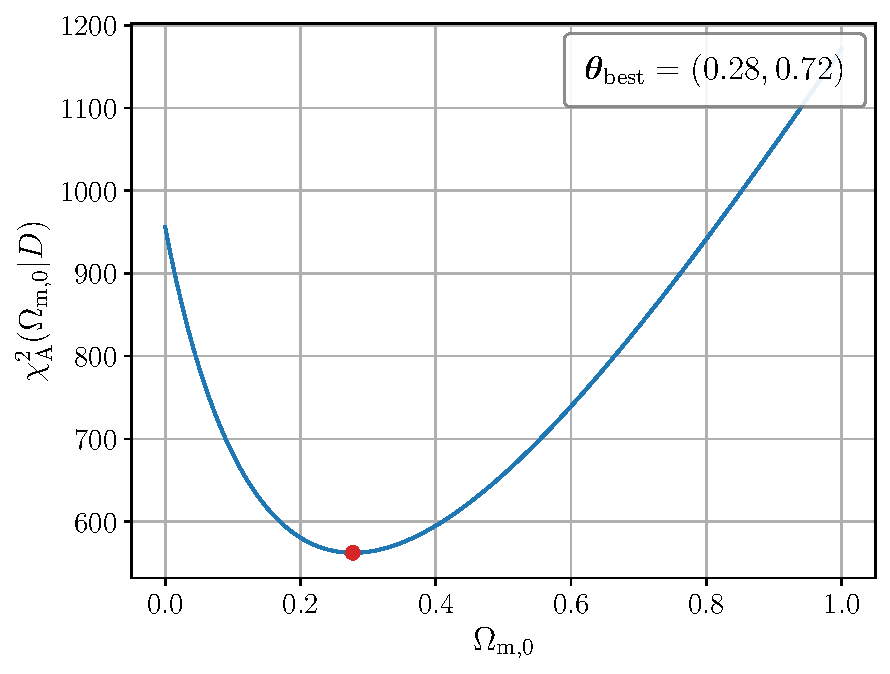
\includegraphics[scale=0.52]{figures/plots/PDF/MWE-analytic-chi2.pdf}
        \caption{Density parameter $\Omega_{\text{m},0}$ vs.\ analytically computed $\chi_{\text{A}}^2(\Omega_{\text{m},0} \vert D)$.}
        \label{fig:MWE-analytic-chi2}
    \end{minipage}
    \hspace*{1cm}
    \begin{minipage}{8cm}
        \centering
        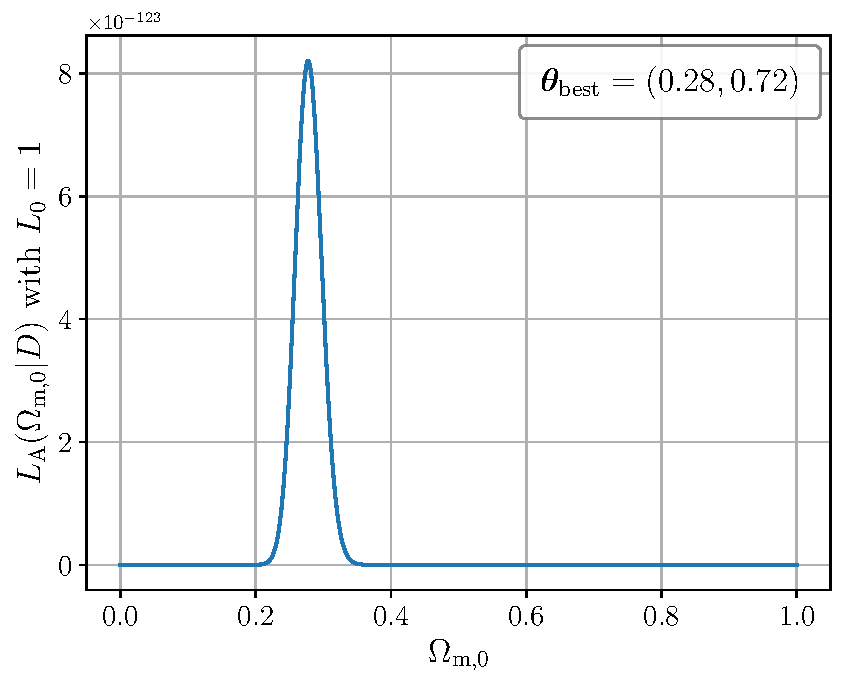
\includegraphics[scale=0.52]{figures/plots/PDF/MWE-analytic-likelihood_L0_1.pdf}
        \caption{Density parameter $\Omega_{\text{m},0}$ vs.\ likelihood $L_{\text{A}}(\Omega_{\text{m},0} \vert D)$ with $L_{0} = 1$.}
        \label{fig:MWE-analytic-likelihood-L0-1}
    \end{minipage}
\end{figure}


\noindent Before calculating the marginalized likelihood $L_{\text{M}}(\Omega_{\text{m},0} \vert D)$, let us compute the likelihood \\
$L(\mathcal{M}, \Omega_{\text{m},0} \vert D)$ (see Equation \ref{eq:likelihood}). To do so, we implement the $\chi^2$-distribution according to Equation \ref{eq:chi-square} as in Listing \ref{lst:chi-square}. Since we call \colorbox{backcolor}{\lstinline{mod_luminosity_distance}} which uses \colorbox{backcolor}{\lstinline{integral}} and therefore \colorbox{backcolor}{\lstinline{quad}}, we split the computation of the likelihood in a function \colorbox{backcolor}{\lstinline{l}} which we can provide with \colorbox{backcolor}{\lstinline{@njit}} and another function \colorbox{backcolor}{\lstinline{likelihood}} in which we compute the luminosity distance $\mathcal{D}_{\text{L}}$. 

\begin{lstlisting}[language=Python, caption={Function for $\chi^2(\mathcal{M}, \Omega_{\text{m},0} \vert D)$.}, label={lst:chi-square}]
@njit
def chi_square(magnitudes, error_magnitudes, theoretical_magnitudes):
    return np.sum(np.square((theoretical_magnitudes - magnitudes) / error_magnitudes))

\end{lstlisting}

\begin{lstlisting}[language=Python, caption={Functions for the likelihood $L(\mathcal{M}, \Omega_{\text{m},0} \vert D)$.}, label={lst:likelihood}]
@njit
def l(mod_absolute_magnitude, mod_luminosity_distance, magnitudes, error_magnitudes, L0):
    m_th = theoretical_magnitude(mod_absolute_magnitude, mod_luminosity_distance)
    chi_2 = chi_square(magnitudes, error_magnitudes, m_th)
    return L0 * np.exp(-0.5 * chi_2)


def likelihood(mod_absolute_magnitude, Omega_m0, redshifts, magnitudes, error_magnitudes, L0):
    D_L = mod_luminosity_distance(redshifts, Omega_m0)
    L = l(mod_absolute_magnitude, D_L, magnitudes, error_magnitudes, L0)
    return L
\end{lstlisting}

\noindent For calculating the marginalized likelihood $L_{\text{M}}$, we integrate over all theoretically possible values of $\mathcal{M} \in (-\infty, \infty)$ (see Equation \ref{eq:marginalized-likelihood}). Numerically, we integrate over an interval in which $L(\mathcal{M}, \Omega_{\text{m},0} \vert D)$ does no longer change significantly as a function of $\mathcal{M}$. As we see from the computation of the likelihood $L(\mathcal{M}, \Omega_{\text{m},0} \vert D)$ (see Figure \ref{fig:MWE-likelihood_mod-absolute-magnitude-vs-likelihood-at-Omega-m0-best} and \ref{fig:MWE-likelihood_mod-absolute-magnitude-vs-Omega-m0-vs-likelihood}), the relevant interval can be chosen as $\mathcal{I}_{\mathcal{M}} = [15.7, 15.9]$. 

\begin{figure}
    \begin{minipage}{8cm}
        \centering
        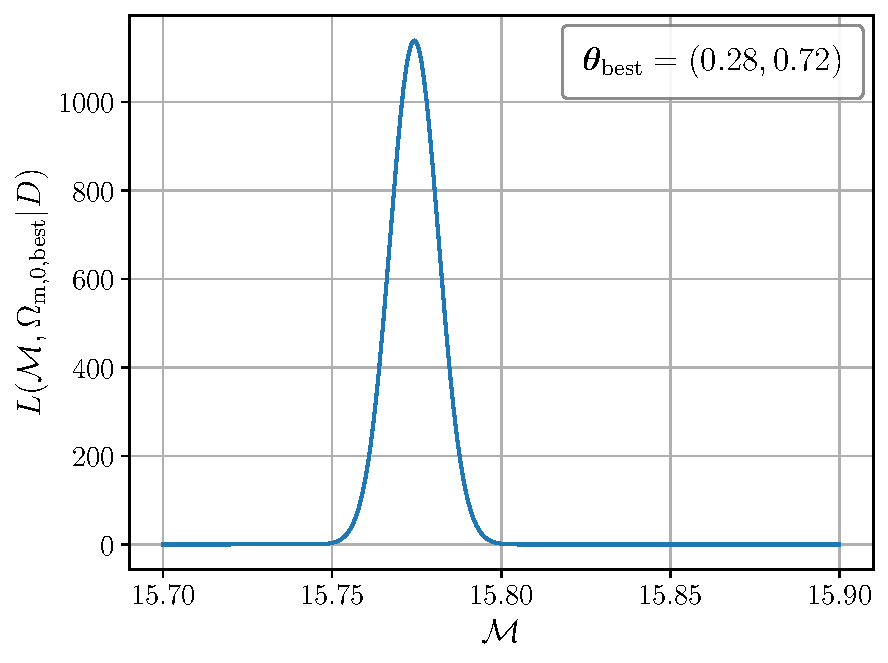
\includegraphics[scale=0.55]{figures/plots/PDF/MWE-likelihood_mod-absolute-magnitude-vs-likelihood-at-Omega-m0-best.pdf}
        \caption{Modified magnitude $\mathcal{M}$ vs.\ likelihood $L(\mathcal{M}, \Omega_{\text{m}, 0, \text{best}} \vert D)$ at $\Omega_{\text{m}, 0, \text{best}} = 0.28$.}
        \label{fig:MWE-likelihood_mod-absolute-magnitude-vs-likelihood-at-Omega-m0-best}
    \end{minipage}
    \hspace*{1cm}
    \begin{minipage}{8cm}
        \centering
        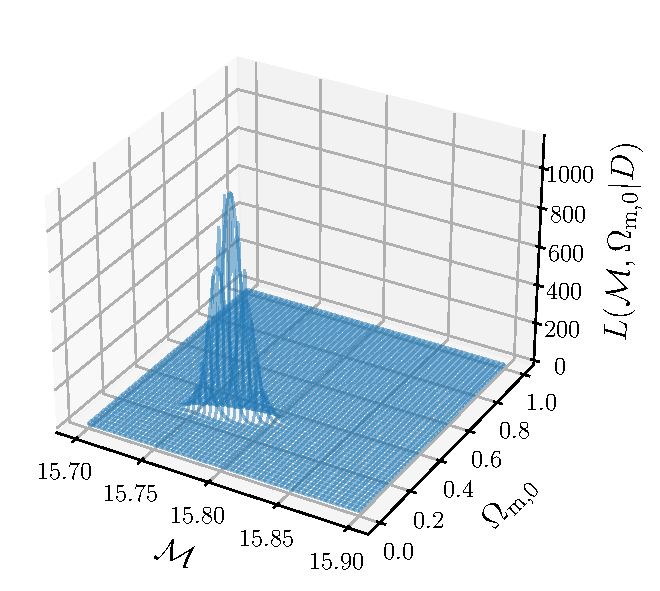
\includegraphics[scale=0.66]{figures/plots/PDF/MWE-likelihood_mod-absolute-magnitude-vs-Omega-m0-vs-likelihood.pdf}
        \caption{Modified magnitude $\mathcal{M}$ vs.\ density parameter $\Omega_{\text{m},0}$ vs.\ likelihood $L(\mathcal{M}, \Omega_{\text{m},0} \vert D)$.}
        \label{fig:MWE-likelihood_mod-absolute-magnitude-vs-Omega-m0-vs-likelihood}
    \end{minipage}
\end{figure}

\noindent The marginalized likelihood $L_{\text{M}}(\Omega_{\text{m},0} \vert D)$ can then be computed as in Listing \ref{lst:marginalized-likelihood}.

\begin{lstlisting}[language=Python, caption={Function for the marginalized likelihood $L_{\text{M}}(\Omega_{\text{m},0} \vert D)$.}, label={lst:marginalized-likelihood}]
def marginalized_likelihood(Omega_m0, redshifts, magnitudes, error_magnitudes, L0):
    D_L = mod_luminosity_distance(redshifts, Omega_m0)
    min_mod_absolute_magnitude = 15.7
    max_mod_absolute_magnitude = 15.9
    margin_L = quad(l, min_mod_absolute_magnitude, max_mod_absolute_magnitude, args=(D_L, magnitudes, error_magnitudes, L0))[0]
    return margin_L
\end{lstlisting}

\begin{figure}[H]
    \begin{minipage}{8cm}
        \centering
        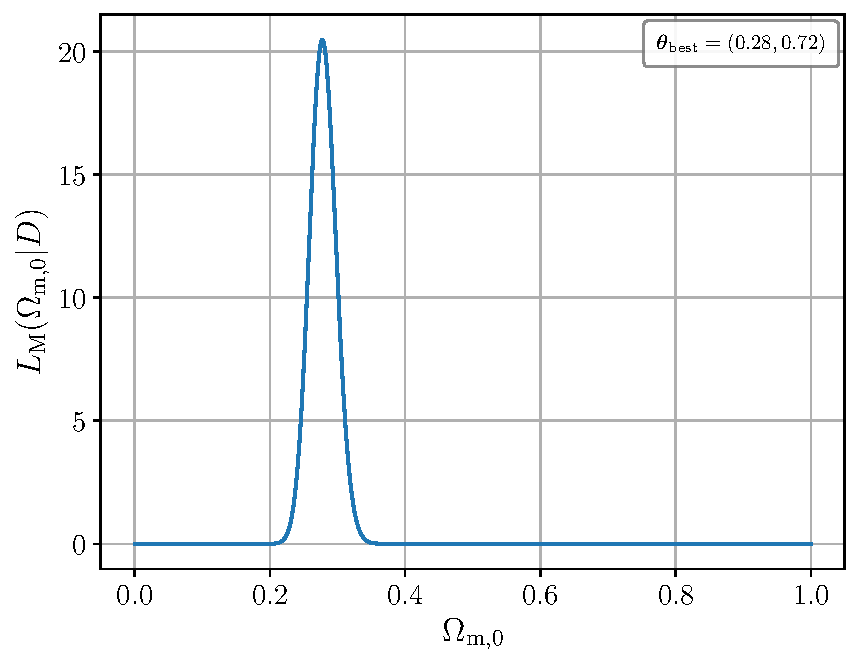
\includegraphics[scale=0.52]{figures/plots/PDF/MWE-marginalized-likelihood.pdf}
        \caption{Density parameter $\Omega_{\text{m},0}$ vs.\ marginalized likelihood $L_{\text{M}}(\Omega_{\text{m},0} \vert D)$.}
        \label{fig:MWE-marginalized-likelihood}
    \end{minipage}
    \hspace*{1cm}
    \begin{minipage}{8cm}
        \centering
        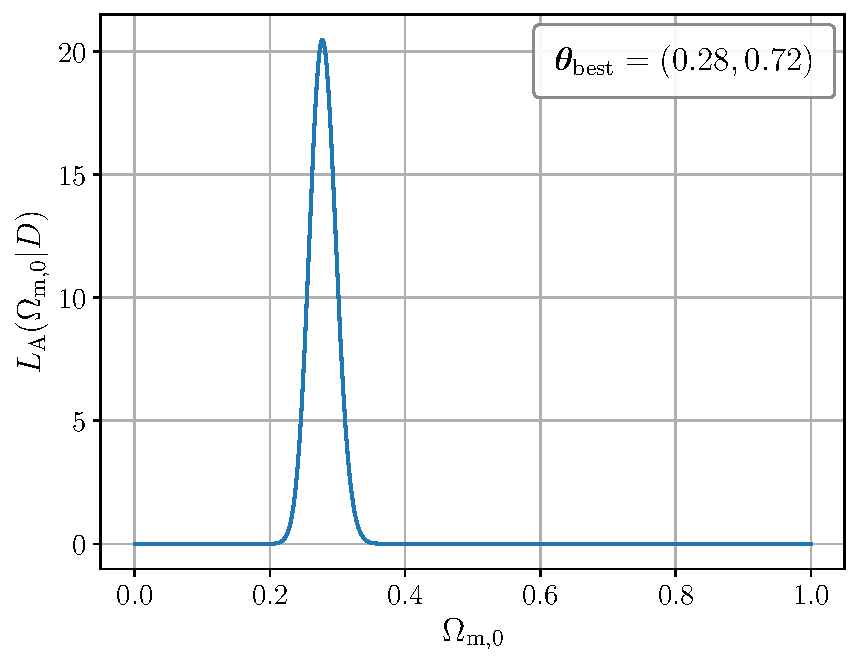
\includegraphics[scale=0.52]{figures/plots/PDF/MWE-analytic-likelihood.pdf}
        \caption{Density parameter $\Omega_{\text{m},0}$ vs.\ analytic likelihood $L_{\text{A}}(\Omega_{\text{m},0} \vert D)$.}
        \label{fig:MWE-analytic-likelihood}
    \end{minipage}
\end{figure}

\noindent As we compare the results for the marginalized likelihood $L_{\text{M}}(\Omega_{\text{m}, 0} \vert D)$ and the analytic likelihood $L_{\text{A}}(\Omega_{\text{m}, 0} \vert D)$ in the Figures \ref{fig:MWE-marginalized-likelihood} and \ref{fig:MWE-analytic-likelihood}, we see that both likelihoods are the same and lead to the same values for the parameter estimation $\vb*{\theta}_{\text{best}} = (\Omega_{\text{m}, 0, \text{best}}, \Omega_{\Lambda, 0, \text{best}}) = (0.28, 0.72)$ (rounded to two decimal places), as we have expected.

\noindent Nevertheless, the sharp pulse shape of the likelihood could lead to incorrect integration as mentioned in the \colorbox{backcolor}{\lstinline{quad}}-documentation, since the size of the function that is integrated compared to the integration interval is important to compute correct values. Therefore, we are going to calculate the $\chi^{2}$-distribution analytically for the evaluation of the $\Lambda$CDM-model in the case of an arbitrary curvature parameter $\Omega_{k,0}$ and for the valuation of the DGP-model.


\subsubsection{$\Lambda$CDM-Model with an Arbitrary Curvature Parameter $\Omega_{k,0}$}

By allowing an arbitrary curvature parameter $\Omega_{k,0} = 1 - \Omega_{\text{m},0} - \Omega_{\Lambda,0}$, the expansion function is given by 
\begin{align}
    E(z) = \sqrt{\Omega_{\text{m}, 0} (1 + z)^3 + (1 - \Omega_{\text{m},0} - \Omega_{\Lambda,0})(1 + z)^2 + \Omega_{\Lambda,0}}. \label{eq:expansion-function-arbitrary-curvature} 
\end{align}

\noindent Further, we need to take the cases of $\Omega_{k,0} < 0$ and $\Omega_{k,0} > 0$ into account when computing the (modified) luminosity distance $\mathcal{D}_{\text{L}}(z, \Omega_{\text{m},0}, \Omega_{\Lambda,0})$ (see Equations \eqref{eq:comoving-distance}, \eqref{eq:expansion-integral}, \eqref{eq:luminosity-distance} and \eqref{eq:relative-magnitude_mod-magnitude_mod-luminosity-distance}). 
First, let us have a look at the computed results for the analytically calculated $\chi^2$-distribution (see Listing \ref{lst:MWE-theoretical-magnitude-and-analytic-chi-square-and-analytic-likelihood}).

\begin{figure}[H]
    \centering
    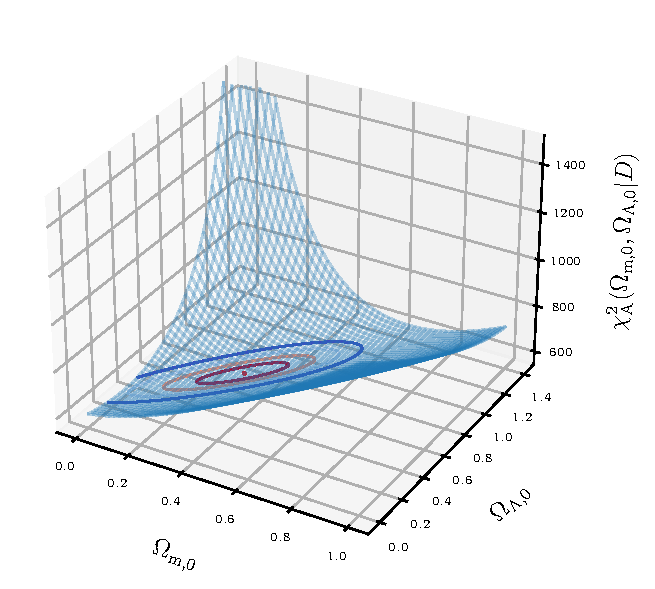
\includegraphics[scale=1.3]{figures/plots/PDF/Lambda-CDM-analytic-chi2_Omega-m0-vs-Omega-Lambda0-vs-chi2.pdf}
    \caption{Density parameters $\Omega_{\text{m},0}$ vs.\ $\Omega_{\Lambda,0}$ vs.\ analytic $\chi_{\text{A}}^2(\Omega_{\text{m},0}, \Omega_{\Lambda,0} \vert D)$.}
    \label{fig:Lambda-CDM-analytic-chi2_Omega-m0-vs-Omega-Lambda0-vs-chi2}
\end{figure}


\begin{figure}
    \begin{minipage}{8cm}
        \centering
        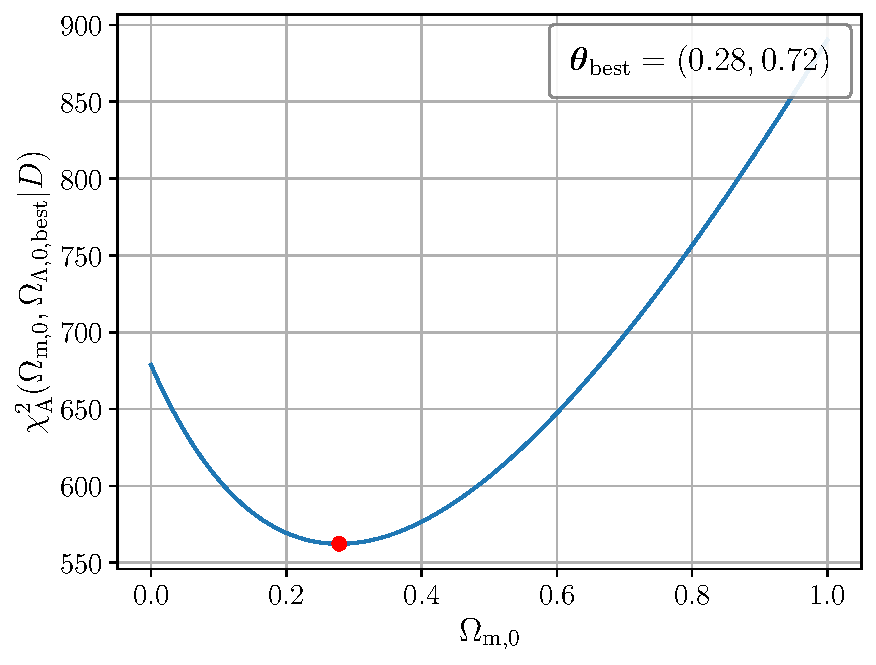
\includegraphics[scale=0.52]{figures/plots/PDF/Lambda-CDM-analytic-chi2_Omega-m0-vs-chi2-at-Omega-Lambda0-best.pdf}
        \caption{Density parameter $\Omega_{\text{m},0}$ vs.\ analytic $\chi_{\text{A}}^2(\Omega_{\text{m},0}, \Omega_{\Lambda, 0, \text{best}} \vert D)$ at $\Omega_{\Lambda, 0, \text{best}} = 0.72$.}
        \label{fig:Lambda-CDM-analytic-chi2_Omega-m0-vs-chi2-at-Omega-Lambda0-best}
    \end{minipage}
    \hspace*{1cm}
    \begin{minipage}{8cm}
        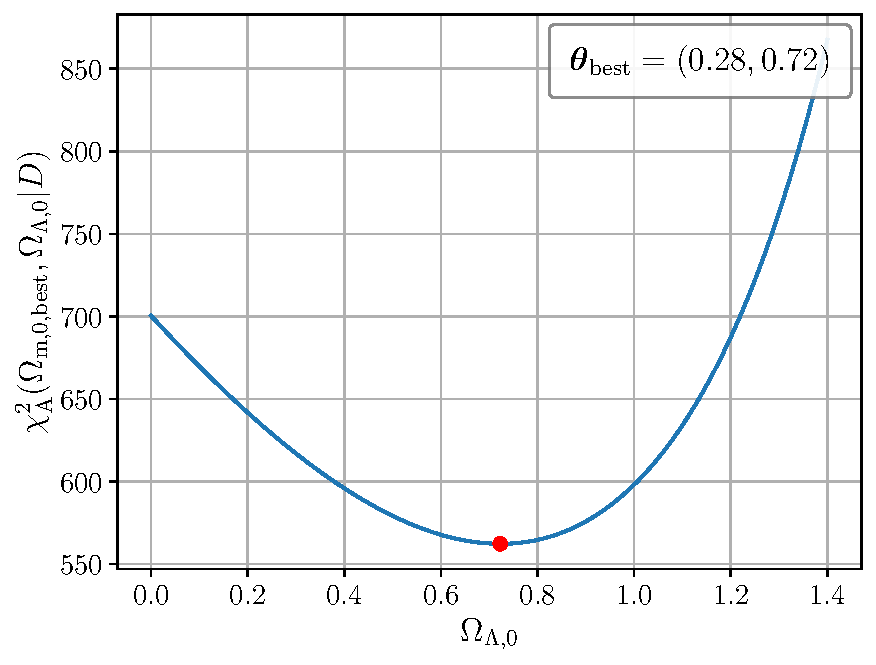
\includegraphics[scale=0.52]{figures/plots/PDF/Lambda-CDM-analytic-chi2_Omega-Lambda0-vs-chi2-at-Omega-m0-best.pdf}
        \caption{Density parameter $\Omega_{\Lambda,0}$ vs.\ analytic $\chi_{\text{A}}^2(\Omega_{\text{m}, 0, \text{best}}, \Omega_{\Lambda, 0} \vert D)$ at $\Omega_{\text{m}, 0, \text{best}} = 0.28$.}
        \label{fig:Lambda-CDM-analytic-chi2_Omega-Lambda0-vs-chi2-at-Omega-m0-best}
    \end{minipage}
\end{figure}

\noindent We obtain for the best-fit values of the $\Lambda$CDM-model with an arbitrary curvature \\
${\vb*{\theta}_{\text{best}} = (\Omega_{\text{m}, 0, \text{best}}, \Omega_{\Lambda, 0, \text{best}}) = (0.28, 0.72)}$.

\begin{figure}[H]
    \centering
    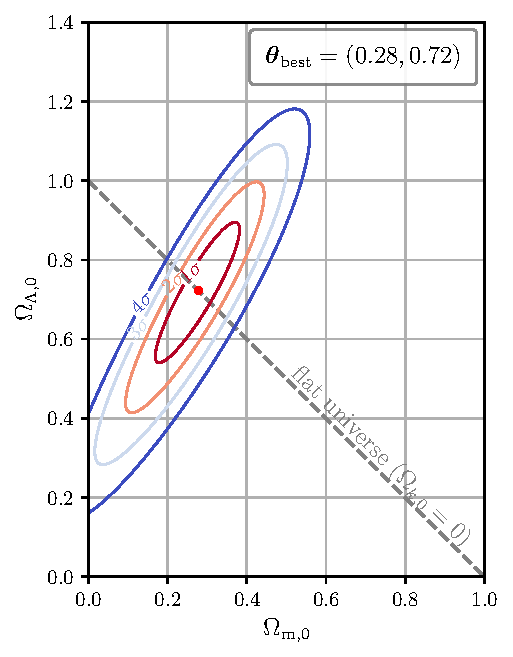
\includegraphics[scale=1.25]{figures/plots/PDF/Lambda-CDM-analytic-chi2_Omega-m0-vs-Omega-Lambda0.pdf}
    \caption{Density parameters $\Omega_{\text{m},0}$ vs.\ $\Omega_{\Lambda,0}$ with calculated $\sigma_{\vb*{\theta}}$-regions by computing $\chi_{\text{A}}^2(\Omega_{\text{m},0}, \Omega_{\Lambda,0} \vert D)$.}
    \label{fig:Lambda-CDM-analytic-chi2_Omega-m0-vs-Omega-Lambda0}
\end{figure}

\noindent To calculate $\sigma$-values for the \text{individual} parameters, we sum the (analytic) likelihood calculated for discrete values of $\vb*{\theta} \in \mathcal{I}_{\vb*{\theta}, n} = [\vb*{\theta}_{\text{min}}, \vb*{\theta}_{\text{max}}, n]$ where $n$ is the amount of linear spaced points between $\vb*{\theta}_{\text{min}}$ and $\vb*{\theta}_{\text{max}}$ such that the dependency of the likelihood $L_{\text{A}} (\vb*{\theta} \vert D)$ is reduced to one parameter. We denote
\begin{align}
    L_{\text{A}, \sum \Omega_{\Lambda,0}}(\Omega_{\text{m}, 0} \vert D) &:= \sum_{\Omega_{\Lambda, 0} \in \mathcal{I}_{\Omega_{\Lambda,0}, n}} L_{\text{A}}(\Omega_{\text{m}, 0}, \Omega_{\Lambda,0} \vert D), \\
    L_{\text{A}, \sum \Omega_{\text{m},0}} (\Omega_{\Lambda, 0} \vert D) &:= \sum_{\Omega_{\text{m}, 0} \in \mathcal{I}_{\Omega_{\text{m},0}, n}} L_{\text{A}}(\Omega_{\text{m}, 0}, \Omega_{\Lambda,0} \vert D)
\end{align}
This to one parameter reduced likelihood has the shape of a (one dimensional) Gaussian curve. Its standard deviation is considered as the $\sigma$-value for the individual parameter. \\
We obtain this $\sigma$-value by fitting a Gaussian curve with \colorbox{backcolor}{\lstinline{scipy.optimize.curve_fit}}\footnote{Documentation of \colorbox{backcolor}{\lstinline{scipy.optimize}}-package: \href{https://docs.scipy.org/doc/scipy/reference/optimize.html}{https://docs.scipy.org/doc/scipy/reference/optimize.html}} for the computed, reduced likelihood.

\begin{figure}[H]
    \centering
    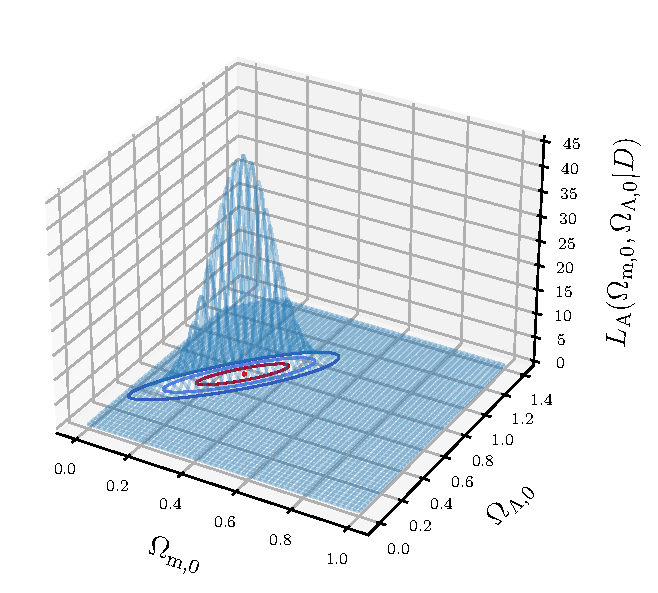
\includegraphics[scale=0.72]{figures/plots/PDF/Lambda-CDM-analytic-likelihood_Omega-m0-vs-Omega-Lambda0-vs-likelihood.pdf}
    \caption{Density parameters $\Omega_{\text{m},0}$ vs.\ $\Omega_{\Lambda,0}$ vs.\ analytic likelihood $L_{\text{A}}(\Omega_{\text{m},0}, \Omega_{\Lambda,0} \vert D)$.}
    \label{fig:Lambda-CDM-analytic-likelihood_Omega-m0-vs-Omega-Lambda0-vs-likelihood}
\end{figure}


\begin{figure}[H]
   \begin{minipage}{8cm}
      \centering
      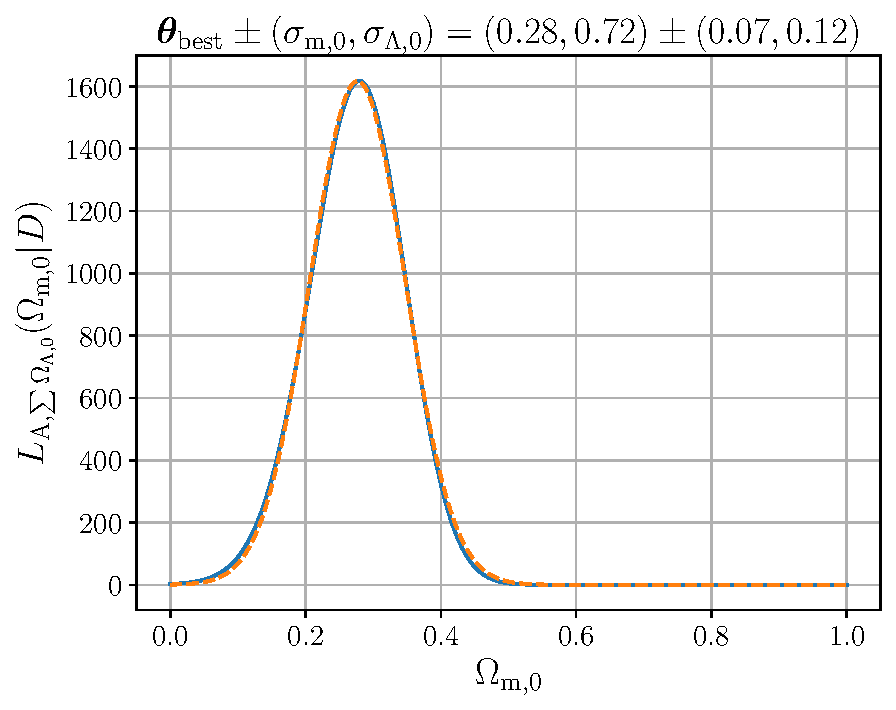
\includegraphics[scale=0.52]{figures/plots/PDF/Lambda-CDM-analytic-likelihood_Omega-m0-vs-likelihood-summed-Omega-Lambda0.pdf}
      \caption{Density parameters $\Omega_{\text{m},0}$ vs.\ reduced, analytic likelihood $L_{\text{A}, \sum \Omega_{\Lambda,0}}(\Omega_{\text{m},0} \vert D)$ and its fit.}
      \label{fig:Lambda-CDM-analytic-likelihood_Omega-m0-vs-likelihood-summed-Omega-Lambda0}
   \end{minipage}
   \hspace*{1cm}
   \begin{minipage}{8cm}
      \centering
      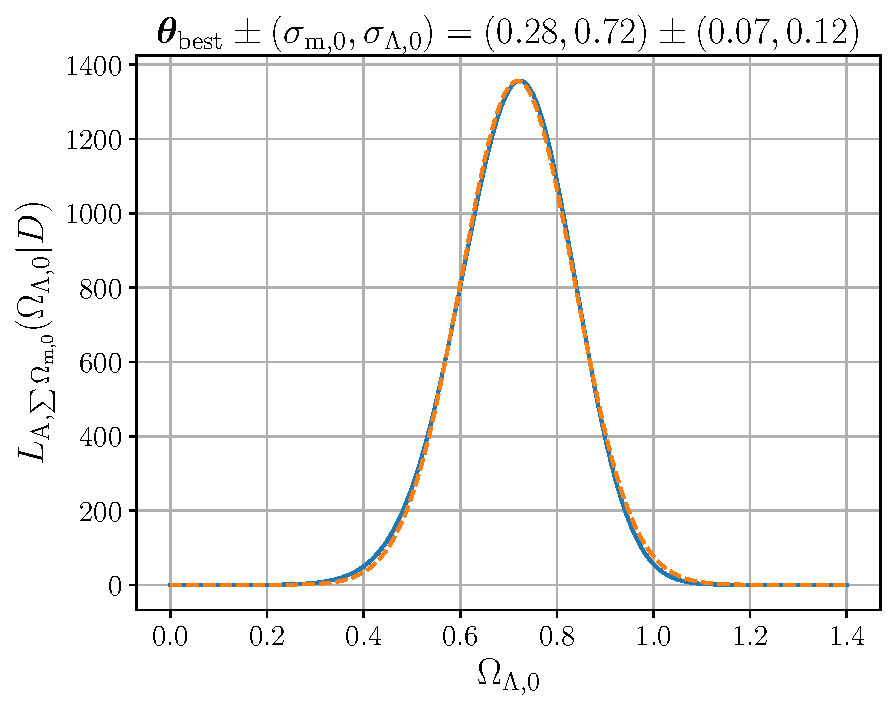
\includegraphics[scale=0.52]{figures/plots/PDF/Lambda-CDM-analytic-likelihood_Omega-Lambda0-vs-likelihood-summed-Omega-m0.pdf}
      \caption{Density parameters $\Omega_{\Lambda,0}$ vs.\ reduced, analytic likelihood $L_{\text{A}, \sum \Omega_{\text{m},0}}(\Omega_{\Lambda,0} \vert D)$ and its fit.}
      \label{fig:Lambda-CDM-analytic-likelihood_Omega-Lambda0-vs-likelihood-summed-Omega-m0}
   \end{minipage}
\end{figure}

\begin{figure}[H]
    \begin{minipage}{8cm}
       \centering
       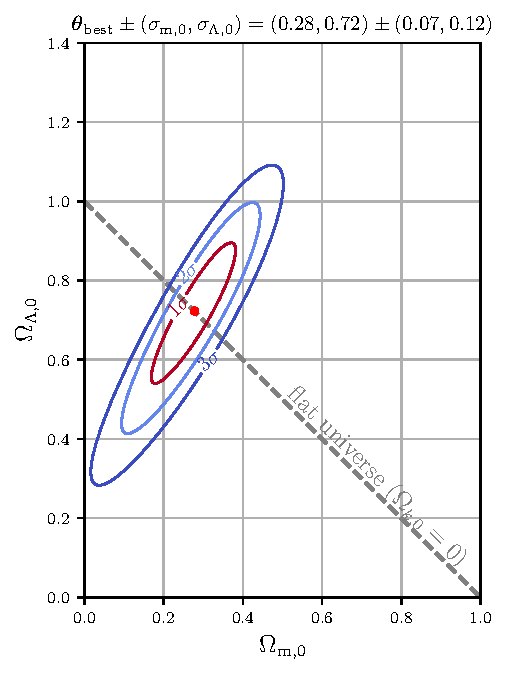
\includegraphics[scale=1.0]{figures/plots/PDF/Lambda-CDM-analytic-likelihood_Omega-m0-vs-Omega-Lambda0.pdf}
       \caption{Density parameters $\Omega_{\text{m},0}$ vs.\ $\Omega_{\Lambda,0}$ with calculated $\sigma_{\vb*{\theta}}$-regions by computing the analytic likelihood $L_{\text{A}}(\Omega_{\text{m},0}, 
       \Omega_{\Lambda,0} \vert D)$.}
       \label{fig:Lambda-CDM-analytic-likelihood_Omega-m0-vs-Omega-Lambda0}
    \end{minipage}
    \hspace*{1cm}
    \begin{minipage}{8cm}
       \centering
       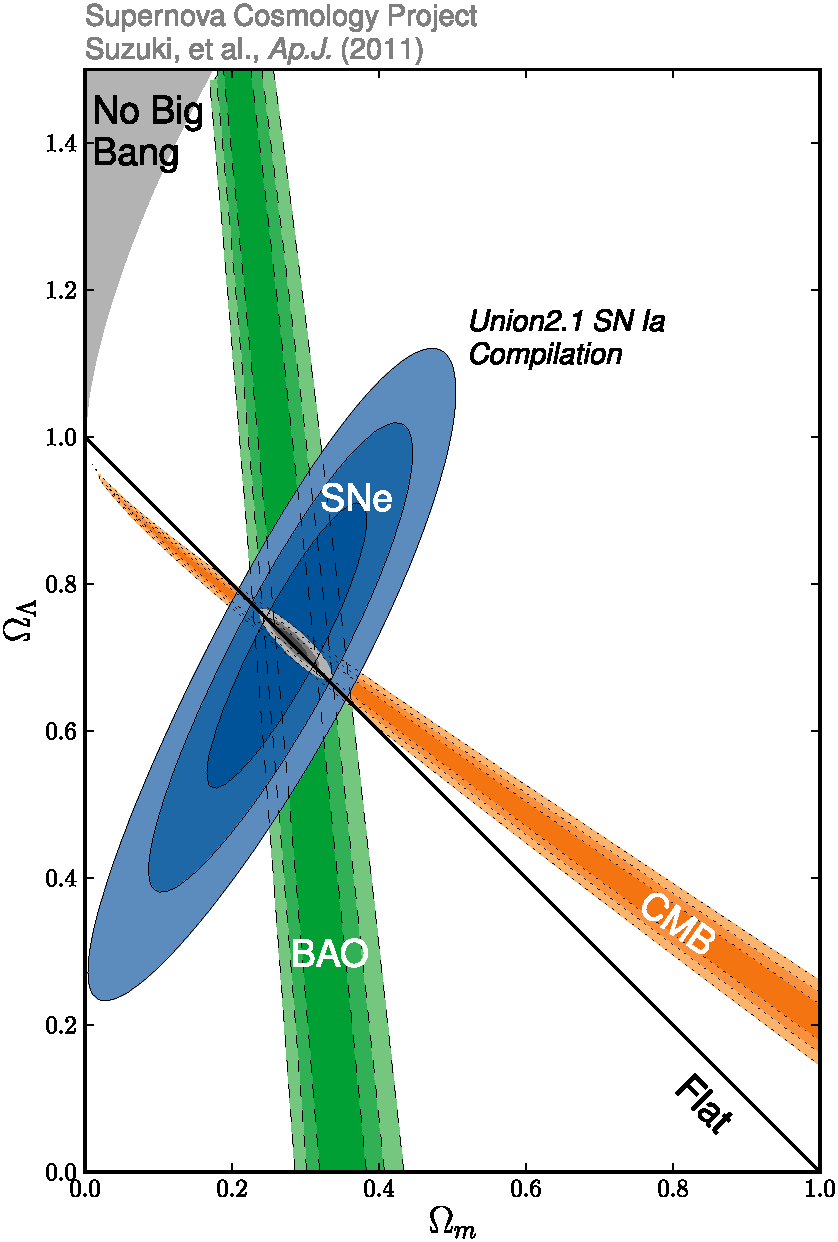
\includegraphics[scale=0.53]{figures/plots/PDF/Union2.1_Om-Ol_slide.pdf}
       \caption{Density parameters $\Omega_{\text{m},0}$ vs.\ $\Omega_{\Lambda,0}$ with calculated $\sigma_{\vb*{\theta}}$-regions by the \textit{Supernova Cosmology Project}. \\
       Source: \cite[Figure 5]{Suzuki2012}}
       \label{fig:Union2.1_Om-Ol_slide}
    \end{minipage}
\end{figure}

\noindent Finally, we can specify the best-fit values with errors as
$\vb*{\theta}_{\text{best}} \pm (\sigma_{\text{m},0}, \sigma_{\Lambda,0}) = (0.28, 0.72) \pm (0.07, 0.12)$. As we compare Figures \ref{fig:Lambda-CDM-analytic-likelihood_Omega-m0-vs-Omega-Lambda0} and \ref{fig:Union2.1_Om-Ol_slide}, we can conclude that our method and code (see appendix \ref{app:dataset-and-source-codes}) can reproduce the results by the \textit{Supernovae Cosmology Project}, though the calculated errors for the individual parameters are slightly larger in our case. \\ 
By considering further constraints like measurements of the cosmic microwave background (CMB) or baryonic acoustic oscillations (BAO), it is possible to specify the best-fit values more precisely and reduce their uncertainty significantly (see \cite[Table 7]{Suzuki2012} and \cite[Table 6 and 7]{Planck2020}).


\subsection{DGP-Model}

For the DGP-model, we implement the modified Friedmann Equations (see Equation \ref{eq:dgp-friedmann-interpolation}) and its derivative with respect to $z$ assuming $z = \text{const.}$ as in Listing \ref{lst:dgp-friedmann-interpolation}. 
\begin{lstlisting}[language=Python, caption={Function for modified Friedmann Equation and its derivative assuming $z = \text{const}$.}, label={lst:dgp-friedmann-interpolation}]
@njit
def mod_friedmann(E, z, Omega_m0, alpha):
    return E * E - (1.0 - Omega_m0) * np.power(E, alpha) - Omega_m0 * np.power(1.0 + z, 3)

@njit
def deriv_mod_friedmann(E, _, Omega_m0, alpha):
    return 2.0 * E - alpha * (1.0 - Omega_m0) * np.power(E, alpha - 1.0)
\end{lstlisting}

\noindent To compute the solution of the modified Friedmann Equation for $E(z)$, we use the \colorbox{backcolor}{\lstinline{root}}-function provided by \colorbox{backcolor}{\lstinline{scipy.optimize}} and implement the solution as in Listing \ref{lst:dgp-friedmann-interpolation-solution}.

\begin{lstlisting}[language=Python, caption={Function to find the solution of the modified Friedmann Equation.}, label={lst:dgp-friedmann-interpolation-solution}]
def sol_friedmann(z, Omega_m0, alpha, mod_friedmann, mod_deriv_friedmann):
    # Solves the modified friedmann equation f(z) = 0 for z with exterior derivative mod_deriv_friedmann
    return opt.root(mod_friedmann, 1.0, args=(z, Omega_m0, alpha), jac=mod_deriv_friedmann).x[0]
\end{lstlisting}

\noindent As in the $\Lambda$CDM-model, it is demanded to calculate the (modified) luminosity distance $\mathcal{D}_{\text{L}}$. Since the implemented computation of $E(z)$ as in Listing \ref{lst:dgp-friedmann-interpolation-solution} is not trivial for \colorbox{backcolor}{\lstinline{quad}} to integrate over, we interpolate the integrand by a sample of redshifts $z'$ and the expansion function $E(z')$ that solves Equation \ref{eq:dgp-friedmann-interpolation} for this sample.


\begin{lstlisting}[language=Python, caption={Functions for computation of the (modified) luminosity distance $\mathcal{D}_{\text{L}}$ in the DGP-model.}, label={lst:dgp-computation-mod-luminosity-distance}]
@njit
def interp_integrand(z, sample_redshifts, sample_E):
    if z == 0.0:
        return 1.0

    E = np.interp(z, sample_redshifts, sample_E)
    return 1.0/E

def interp_integral(z, sample_redshifts, sample_E):
    # d_C/d_H = Integrate[1/E(z'), {z', 0, z}]
    return quad(interp_integrand, 0.0, z, args=(sample_redshifts, sample_E))[0]

def mod_luminosity_distance(z, Omega_m0, alpha):
    # Cosmological Parameters
    # =======================
    c = 299792.458           # speed of light in vacuum in km/s
    H_0 = 1.0                # dependence on hubble constant is set into the mod_absolute_magnitude, see theoretical_magnitude
    d_H = c/H_0              # hubble distance
    # =======================
    
    sample_redshifts = np.linspace(0.0, max(z), 1000)
    sample_E = np.array([sol_friedmann(zi, Omega_m0, alpha, mod_friedmann, deriv_mod_friedmann) for zi in sample_redshifts])

    I = np.array([interp_integral(zi, sample_redshifts, sample_E) for zi in z])
    
    return (1.0 + z) * d_H * I
\end{lstlisting}

\noindent Further, we compute the $\chi^2$-distribution analytically as in Listing \ref{lst:MWE-theoretical-magnitude-and-analytic-chi-square-and-analytic-likelihood} and \ref{lst:dgp-chi2}. In the following, we only consider $\chi_{\text{A}}^{2}(\Omega_{\text{m,0}}, \alpha \vert D)$, which is sufficient to estimate best-fit values for $\vb*{\theta} = (\Omega_{\text{m},0}, \alpha)$.

\begin{lstlisting}[language=Python, caption={Function for analytic $\chi_{\text{A}}^2(\Omega_{\text{m},0}, \alpha \vert D)$.}, label={lst:dgp-chi2}]
def chi2(Omega_m0, alpha, redshifts, magnitudes, error_magnitudes):
    mod_absolute_magnitude = 0.0
    D_L = mod_luminosity_distance(redshifts, Omega_m0, alpha)
    m_th = theoretical_magnitude(mod_absolute_magnitude, D_L)
    chi_2 = analytic_chi_square(magnitudes, error_magnitudes, m_th)
    return chi_2  
\end{lstlisting}

\begin{figure}[]
    \begin{minipage}{8cm}
        \centering
        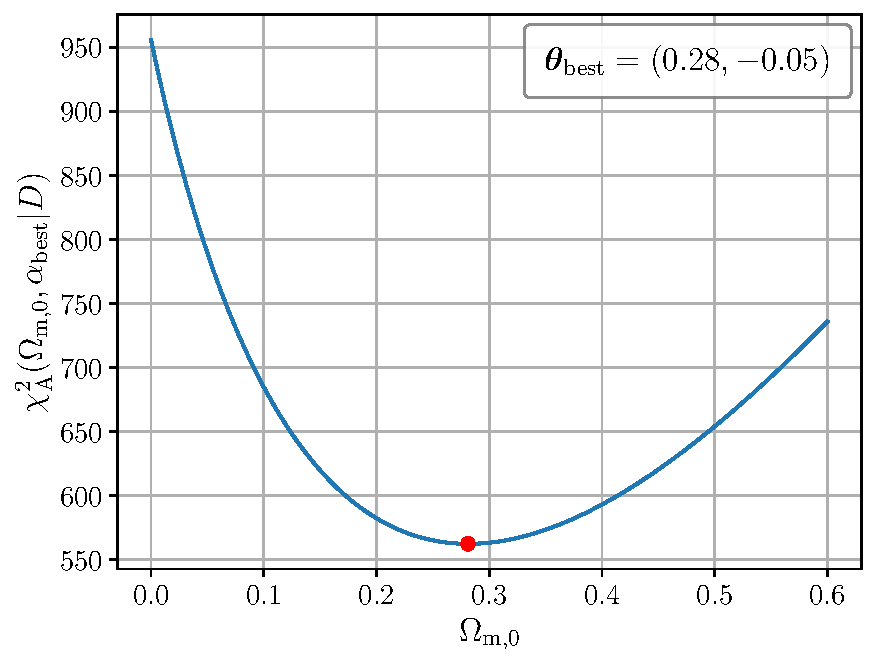
\includegraphics[scale=0.50]{figures/plots/PDF/DGP-analytic-chi2_Omega-m0-vs-chi2-at-alpha-best.pdf}
        \caption{Density parameter $\Omega_{\text{m},0}$ vs.\ analytic $\chi_{\text{A}}^2(\Omega_{\text{m},0}, \alpha_{\text{best}} \vert D)$ at $\alpha_{\text{best}} = -0.05$.}
        \label{fig:DGP-analytic-chi2_Omega-m0-vs-chi2-at-alpha-best}
    \end{minipage}
    \hspace*{0.5cm}
    \begin{minipage}{8.2cm}
       \centering
       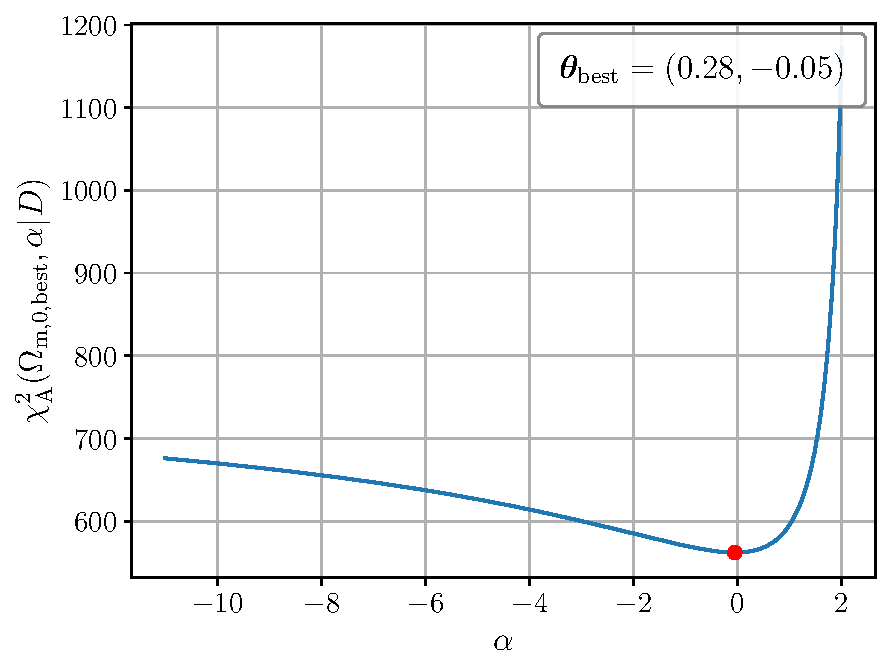
\includegraphics[scale=0.50]{figures/plots/PDF/DGP-analytic-chi2_alpha-vs-chi2-at-Omega-m0-best.pdf}
       \caption{Interpolation parameter $\alpha$ vs.\ analytic $\chi_{\text{A}}^2(\Omega_{\text{m}, 0, \text{best}}, \alpha \vert D)$ at $\Omega_{\text{m}, 0, \text{best}} = 0.28$.}
       \label{fig:DGP-analytic-chi2_alpha-vs-chi2-at-Omega-m0-best}
    \end{minipage}
\end{figure}

\begin{figure}[H]
    \centering
    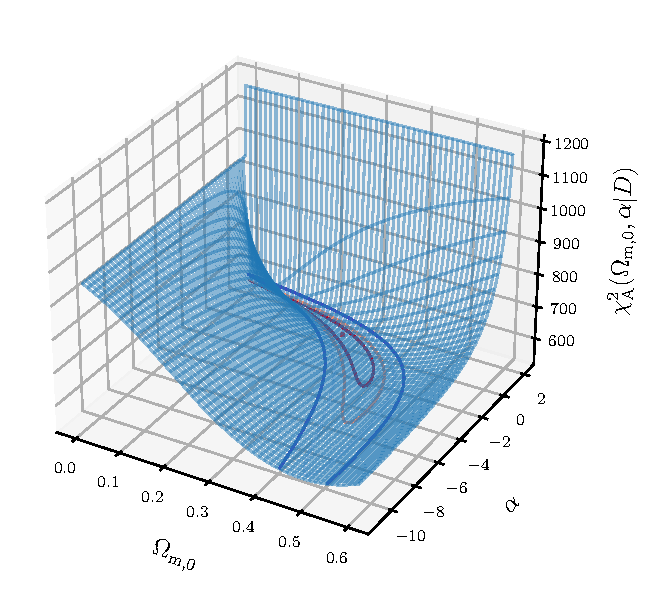
\includegraphics[scale=1.0]{figures/plots/PDF/DGP-analytic-chi2_Omega-m0-vs-alpha-vs-chi2.pdf}
    \caption{Density parameter $\Omega_{\text{m},0}$ vs.\ interpolation parameter $\alpha$ vs.\ analytic $\chi_{\text{A}}^2(\Omega_{\text{m},0}, \alpha \vert D)$.}
    \label{fig:DGP-analytic-chi2_Omega-m0-vs-alpha-vs-chi2}
\end{figure}

\noindent Finally, we obtain for the best-fit values $\vb*{\theta}_{\text{best}} = (0.28, -0.05)$. 
As we see in Figure \ref{fig:DGP-analytic-chi2_Omega-m0-vs-alpha-vs-chi2} and Figure \ref{fig:DGP-analytic-chi2_Omega-m0-vs-alpha-full}, the $\sigma_{\vb*{\theta}}$-regions spread out broadly in parameter space as the $\chi^2$-distribution flattens. This makes it difficult to give an adequate estimate of the $\sigma$-uncertainties for the individual parameters. Nevertheless, we can conclude that this parameter estimation of $\vb*{\theta} = (\Omega_{\text{m},0}, \alpha)$ tends to prefer the $\Lambda$CDM-model (for which $\alpha = 0$) over the DGP-model (for which $\alpha = 1$). As shown in Figure \ref{fig:testing-DGP-with-planck} (see \cite[Figure 3]{Li2013}), accounting multiple datasets such as measurements of baryonic acoustic oscillations (BAO) or cosmic microwave background (Planck), but also measurements of weak gravitational lensing (see \cite[Figure 7]{Thomas2009}) allow constraints that disfavour the DGP-model.

\begin{figure}[]
    \centering
    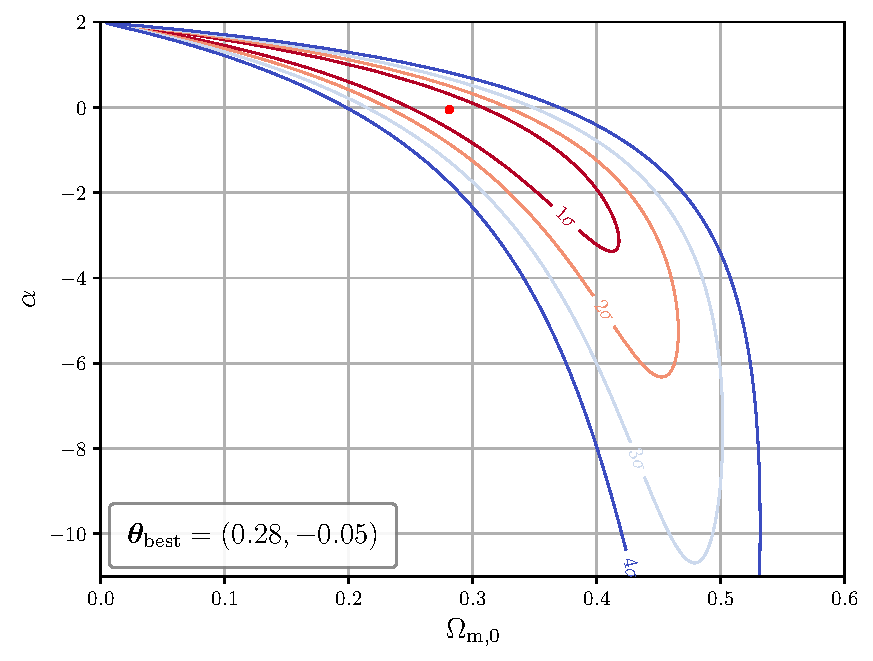
\includegraphics[scale=1.0]{figures/plots/PDF/DGP-analytic-chi2_Omega-m0-vs-alpha-full.pdf}
    \caption{Density parameter $\Omega_{\text{m},0}$ vs.\ interpolation parameter $\alpha$ with calculated $\sigma_{\vb*{\theta}}$-regions by computing $\chi_{\text{A}}^2(\Omega_{\text{m},0}, \alpha \vert D)$.}
    \label{fig:DGP-analytic-chi2_Omega-m0-vs-alpha-full}
\end{figure}

\begin{figure}
    \begin{minipage}{8cm}
        \centering
        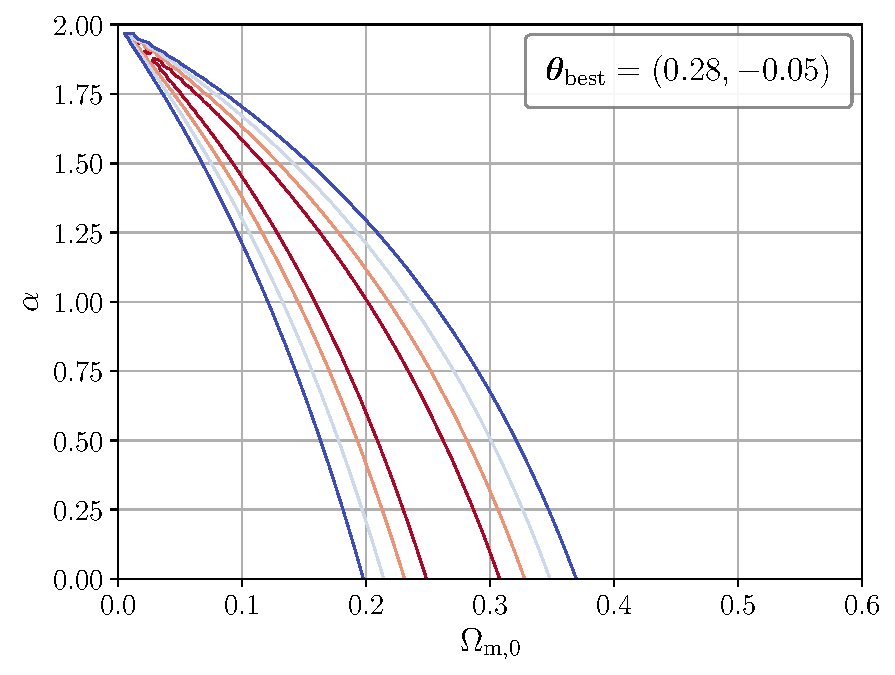
\includegraphics[scale=0.53]{figures/plots/PDF/DGP-analytic-chi2_Omega-m0-vs-alpha-0-2.pdf}
        \caption{Density parameter $\Omega_{\text{m},0}$ vs.\ interpolation parameter $\alpha$ with calculated $\sigma_{\vb*{\theta}}$-regions for $\alpha \in [0.0, 2.0]$.}
        \label{fig:DGP-analytic-chi2_Omega-m0-vs-alpha-0-2}
    \end{minipage}
    \hspace*{1cm}
    \begin{minipage}{8cm}
        \centering
        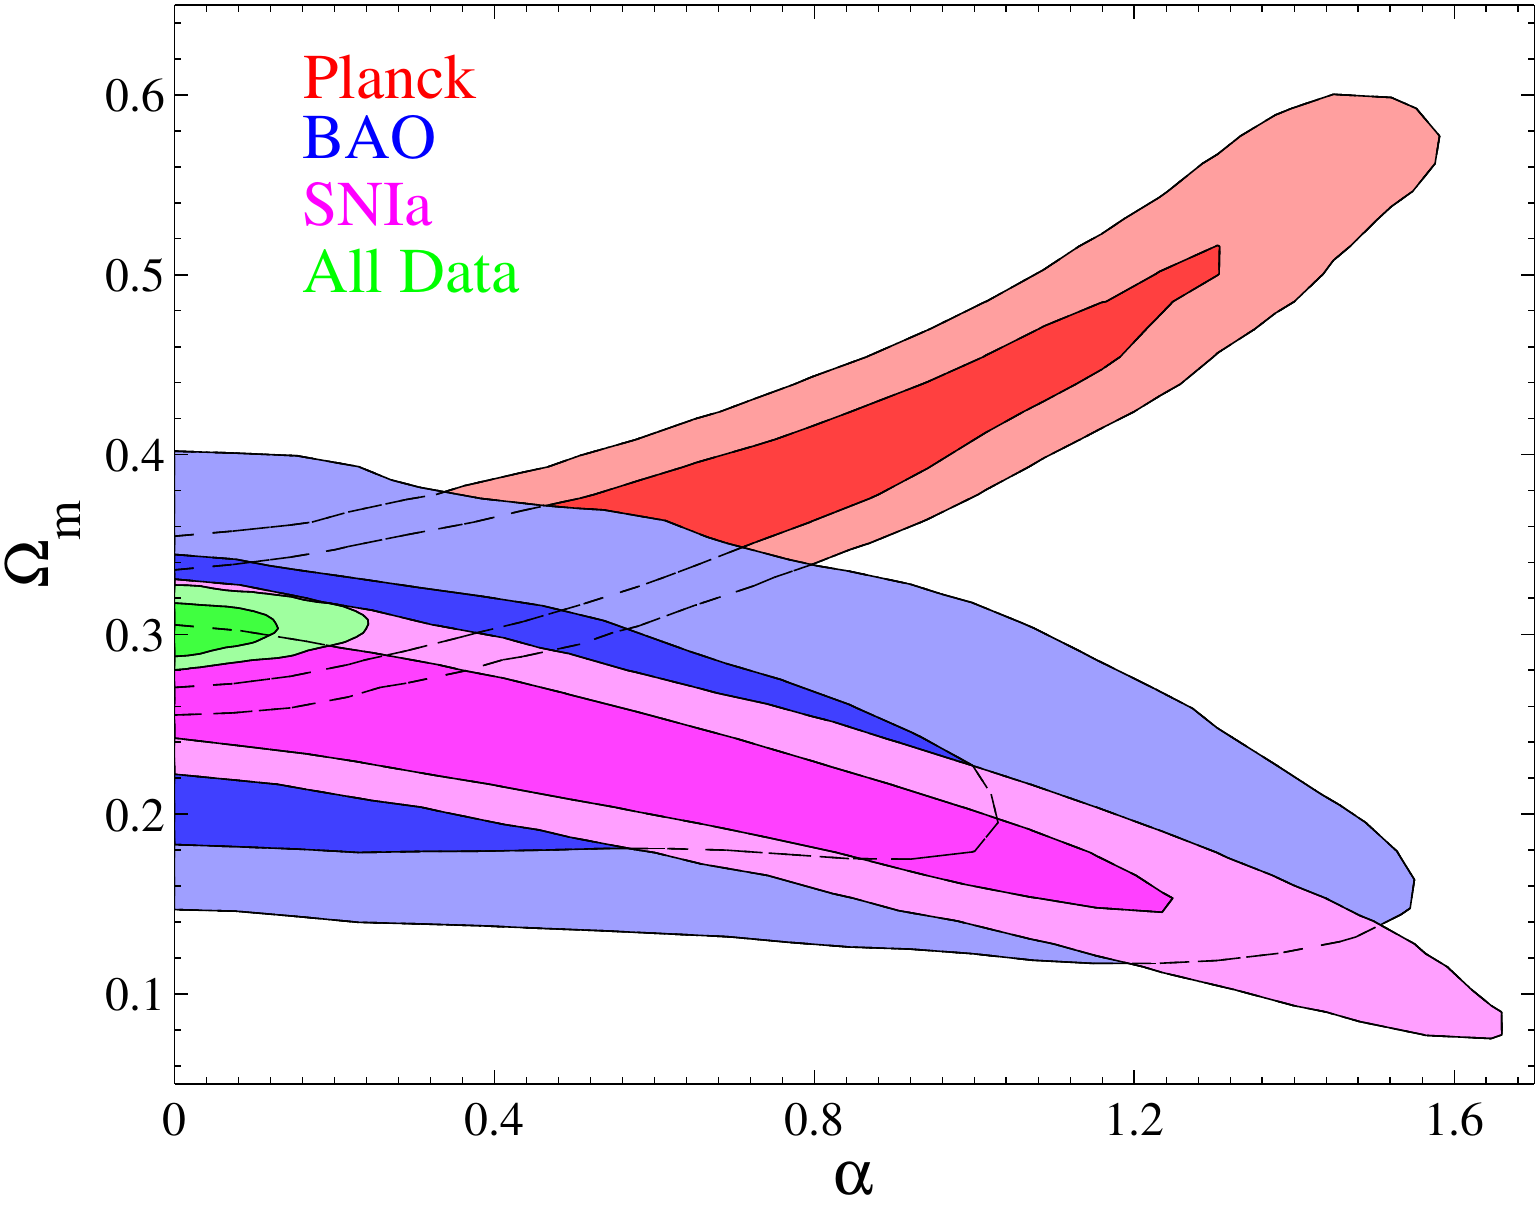
\includegraphics[scale=0.55]{figures/plots/PNG/testing-DGP-with-planck.png}
        \caption{Density parameter $\Omega_{\text{m},0}$ vs.\ interpolation parameter $\alpha$ considering several cosmological constraints. \\
        Source: \cite[Figure 3]{Li2013}}
        \label{fig:testing-DGP-with-planck} 
    \end{minipage}
\end{figure}


